\capitulo{4}{Técnicas y herramientas}

\section{Metodologías}
\subsection{SCRUM}

    SCRUM es una metodología ágil basada en una estrategia continua e incremental, cuyo objetivo es proporcionar un producto funcional al final de cada periodo de trabajo planeado (\textit{sprint}), haciendo reuniones diarias y antes y después de cada \textit{sprint} otras reuniones donde se explican los problemas que se han tenido y como se va a planear el siguiente.

    El impedimento más notorio de esta metodología, es que hay un equipo de personas entre las que se encuentra el \textit{product owner}, el \textit{SCRUM master} y el equipo de desarrollo. 
    
    Además se recomienda que el equipo este formado por 3 a un máximo de 9 personas para un buen desarrollo, por tanto, en este trabajo ha sido complicado ir haciendo todas las acciones que se piden en la metodología SCRUM.

\subsection{GitFlow}

    GitFlow es un flujo de trabajo, en el cual se ramifica el proyecto en \textit{branches} donde cada una, contiene una parte del proyecto; de esta forma, se puede dejar una parte funcional sin modificar que sería la rama principal, y otras ramas, donde se van realizando los cambios, cuando en estas ramas, se termina la tarea que se esta realizando, haciendo un producto funcional, se realiza una operación de \textit{pull request} para combinar ambas ramas. Esta operación es aceptada o denegada por el equipo de desarrollo que no haya participado en la realización de esta rama.

    En el proyecto, se han creado tres \textit{branches}, que son:
    \begin{itemize}
        \item \textit{main}: es la rama principal, donde se alberga la versión estable del proyecto.
        \item boceto: es una rama secundaria, donde se realizan los cambios que se están realizando en la aplicación móvil.
        \item latex: es la rama secundaria donde se realizan los cambios que se están realizando en el documento LaTeX.
    \end{itemize}
\subsection{Método del pato de goma}

    El método del pato de goma, o \textit{rubber duck debugging}~\cite{rubber-duck-debugging}, es un método informal para la revisión de código.

    Este método es utilizado por muchos programadores y surgió porque normalmente los programadores han tenido experiencias donde han tenido que explicar el problema a otra persona que no entiende sobre programación, y mientras se esta explicando el código, encontrar posibles soluciones. 
    
    Por tanto, este método, consiste en vez de explicar el código a otra persona, en explicárselo a un pato de goma.

\section{Herramientas}

    \subsection{Repositorio}
        Entre las opciones para realizar el repositorio, se pensó en \href{https://gitlab.com/}{GitLab} y en \href{https://github.com/}{GitHub}, tomando esta última por conocimiento de uso de esta.

        GitHub es una plataforma web de alojamiento de repositorios que utiliza \href{https://git-scm.com/}{Git} como sistema de control de versiones.

        Por tanto, como GitHub utiliza \href{https://git-scm.com/}{Git} de forma nativa, no fue necesario la elección de un sistema de control de versiones.

        Como para el repositorio se necesitan archivos de más de 100 MB, se ha usado la extensión \href{https://git-lfs.com/}{Git LFS}, estos ficheros son los las redes neuronales, tanto formato keras, como formato TensorFlow Lite.
    \subsection{Gestión del proyecto}
        Entre las opciones para gestionar el proyecto, se pensó en poder realizarlo con \href{https://github.com/}{GitHub Projects}, con \href{https://www.atlassian.com/es/software/jira}{Jira}, con \href{https://www.zenhub.com/}{ZenHub} y \href{https://trello.com/}{Trello}; tomando la opción de \href{https://www.zenhub.com/}{ZenHub}, por ya estar familiarizado con la herramienta.

        ZenHub es una herramienta de gestión de proyectos que se integra con GitHub. Proporciona una tabla Kanban, donde se ponen las actividades a realizar durante el \textit{sprint}. Permite poner una prioridad a las tareas, siguiendo una estimación de póquer, y además, ofrece la posibilidad de ver gráficos \textit{burndown} donde se representa las actividades que faltan por hacer en el \textit{sprint}, también ofrece otros gráficos como \textit{cumulative flow} y \textit{velocity tracking}.

    \subsection{Guía de diseño}
        Para la realización de la aplicación, es necesario una guía de diseño que facilite al usuario la interacción con la aplicación. Por ello, se utilizo la ultima guía ofrecida por Google, llamada \href{https://m3.material.io/}{Material 3}.

        \href{https://m3.material.io/}{Material 3} es la última versión del sistema de diseño del \textit{open source} de Google.
        En el documento, viene información de recomendación de componentes ante el mismo problema.

    \subsection{Herramienta de iconos}
        Para la adición de iconos en la aplicación, es necesario que las imágenes y o iconos sean \textit{open source} para ello, se estuvieron mirando páginas que ofrecían estos iconos, entre las páginas, al final se seleccionaron \href{https://pixabay.com/es/}{pixabay} para la obtención de imágenes, puesto que ofrece licencia de uso para proyectos comerciales y no comerciales.

        Por otro lado, para los iconos se utilizó \href{https://fonts.google.com/icons}{Google Fonts} y la galería que ofrece Android por defecto, se utilizo \href{https://fonts.google.com/icons}{Google Fonts}, porque en la guía de desarrollo se recomendaba y a su vez, es de código abierto y gratuito.

        Para el logotipo de la aplicación, se ha utilizado \href{https://labs.openai.com/}{DALL-E} , una inteligencia artificial que convierte texto a imágenes, tras varios intentos, se logró conseguir un logotipo bastante bueno, y con ello, se hicieron unos retoques con el uso del programa de edición de imágenes \href{https://www.gimp.org/}{GIMP}, para la eliminación de ruido y para proporcionarle una gamma de colores; como resultado se obtuvo el icono actual.

    \subsection{Entorno de desarrollo integrado (IDE)}
        Para el desarrollo de la aplicación móvil, se pensó en \href{https://www.eclipse.org/downloads/}{Eclipse}, \href{https://developer.android.com/studio}{Android Studio} y \href{https://unity.com/es}{Unity}.

        Al final, se descartó Eclipse por no ofrecer una experiencia de desarrollo especifica para aplicaciones Android. Y también se descarto Unity, aunque Unity si que esta especializado en aplicaciones móviles, por otro lado, se especializa en el desarrollo de videojuegos y en aplicaciones con realidad virtual.
        Por lo tanto, se selecciono Android Studio, es el IDE oficial de Android y está desarrollado por Google, basado en IntelliJ IDEA. Ofrece un emulador donde se compila la aplicación y poder comprobar el correcto funcionamiento de esta.
        Además, para la compilación hace uso de Gradle, separando el código de la aplicación, de la compilación.

        El lenguaje utilizado ha sido Java, aunque Android Studio ofrece la opción de Kotlin, con Java no hacia falta aprender un nuevo lenguaje, puesto que se ha cursado durante la carrera.

    \subsection{LaTeX}
        Para la realización del documento, se pensó utilizar \href{https://miktex.org/}{MiKTeX}, \href{https://www.tug.org/texlive/}{TeX Live} u \href{https://www.overleaf.com/}{Overleaf}.
    
        Al final, se escogió Overleaf, puesto que las otras 2 herramientas eran locales, y Overleaf ofrece acceso desde la nube, además tiene integración con proyectos GitHub, facilitando la exportación al repositorio.
    \subsection{Comunicación}
        Para la comunicación con los tutores, se uso tanto email, como tutorías presenciales, de esta forma, las cuestiones y los avances realizados se hacen por email, y en caso de mostrar el funcionamiento de la aplicación o alguna duda más importante, se realiza presencialmente para un mejor entendimiento.

    \subsection{Librerías}
    
        \subsubsection{Librerías Android Studio}
        \hfill \break
            Para la aplicación Android, se han usado las siguientes librerías:
            \hfill \break
            
            \textbf{AndroidX Appcompat}
            
                Es una librería estática de Android que al añadirla al proyecto permite el uso de funcionalidades no incluidas en el framework o utilizar APIs no disponibles para versiones anteriores. Tiene compatibilidad con versiones de Android con una API 14 o mayor.
        
            \textbf{Material}
            
                Esta librería estática de Android permite implementar las especificaciones incluidas en Material Design. Tiene compatibilidad con versiones de Android con una API 14 o mayor.
                
            \textbf{ConstraintLayout}
            
                Esta librería de Android permite al desarrollador una forma flexible y adaptable de poner los \textit{Widgets}.
        
            \textbf{JUnit}
            
                Es un framework para Java, que permite realizar pruebas unitarias.
                
            \textbf{AndroidX Espresso}
            
                Es un framework de pruebas de interfaz de usuario (UI) para las aplicaciones Android.
                
            \textbf{TensorFlow Lite}
            
                Es una librería de Android que permite desplegar modelos de aprendizaje automático en los dispositivos móviles.
            
            \textbf{SQLite}
            
                Es una librería de Android que permite la integración de bases de datos en dispositivos móviles.
                
    \subsection{Librerías de Python}
    
        Para la creación del modelo se han usado las siguientes librerías:

        \textbf{time}
        
            Es un módulo de la librería estándar de Python que permite trabajar con tiempos.

        \textbf{numpy}
        
            Es una librería de Python que permite manejar \textit{arrays}, álgebra lineal, transformaciones de fourier y matrices.

        \textbf{pandas}
        
            Es una librería de Python que permite analizar, limpiar, explorar y manipular el conjuntos de datos.

        \textbf{Matplotlib}
        
            Es una libreria de python para ver visualmente gráficas de nivel bajo.

        \textbf{sklearn.metrics.confusion\_matrix}
        
             Es una función de la librería de scikit-learn que permite trabajar con matrices de confusión.

        \textbf{tensorflow.keras}
        
            Es un framework de aprendizaje automatico, de este se utilizan varias clases: 
            \begin{itemize}
                \item preprocessing.image.ImageDataGenerator: es una clase de Python que permite diversas transformaciones y aumentos de datos, como rotación, cambio de tamaño, recorte, cambio de brillo, entre otros.
                \item tensorflow.keras.applications.VGG16: es una clase de Python que proporciona la implementación de un modelo VGG16.
                \item tensorflow.keras.applications.VGG16.preprocess\_input: es una función de la clase VGG16 que proporciona el preprocesado de la imagen en un modelo VGG16.
                \item tensorflow.keras.models.Sequential: es una clase de Python que permite agrupar un conjunto de capas, para convertirlas en un modelo.
                \item tensorflow.keras.layers: es un módulo que contiene información sobre las capas.
                \item tensorflow.keras.optimizers.Adam: es una clase que implementa el algoritmo Adam. El cual es un algoritmo de descenso de gradiente estocástico. Siendo un optimizador eficiente con consumo pequeño de recursos.
                \item tf.keras.metrics.Precision: es una clase que permite calcular la precisión de las predicciones con respecto a las etiquetas.
                \item tf.keras.metrics.Recall: es una clase que permite calcular el ``recall'' de las predicciones con respecto a las etiquetas.  
            \end{itemize}
            
        \textbf{sklearn.model\_selection.test\_train\_split}
        
            Es una función de la librería de scikit-learn que permite dividir el conjunto de datos en conjunto de entrenamiento y conjunto de pruebas.
            
        \textbf{os}
        
            Es una librería de Python permite trabajar con funcionalidades del sistema operativo; a su vez se ha usado el módulo path de esta librería, el cual permite obtener la ruta desde donde se esta ejecutando el archivo.
    
\section{Patrones de diseño}
    \subsection{Modelo-Vista-Presentador}
        Es una derivación del patrón modelo-vista-controlador, la diferencia es que se cambia el controlador por un presentador, el cual sirve como intermediario entre el modelo y la interfaz.
        \begin{itemize}
            \item El modelo, define los datos que se utilizan en la interfaz.
            \item El presentador, funciona como intermediario, recuperando los datos del modelo, y cambiando la vista de la interfaz.
            \item La vista, es la interfaz de usuario.
        \end{itemize}
        
        Puesto que Android Studio, ya proporciona separaciones para hacer uso de un modelo-vista-presentador, su implementación ha sido sencilla, donde las \textit{activities} son las diferentes interfaces, los archivos java del directorio ``com.example.retinopatia'' son los presentadores de las vistas, y en el directorio DataBase se encuentra el modelo de datos.

        En la figura \ref{fig:modeloVistaPresentador}, se puede observar su funcionamiento.
        \begin{figure}[!ht]
                 \centering
                 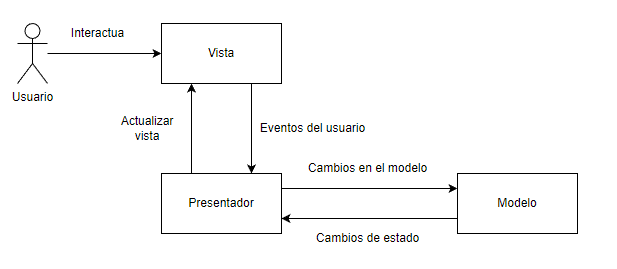
\includegraphics[width=0.9\textwidth]{img/MVP.png}
                  \caption{Modelo-Vista-Presentador}
                 \label{fig:modeloVistaPresentador}
        \end{figure}
    \subsection{Patrón singleton}
        Este patrón sirve para restringir la creación de objetos. En el caso utilizado, ha sido para la base de datos, de esta forma, no se creaba de cero cada vez que se iniciaba la aplicación.
